%%____________________________________________________________________________||
\section{Results}
\label{sec:results}

The following section summarises the result of this analysis. The
control regions are populated with the full data set of 2016, namely
35.9\fbinv. As indicated in Sec.~\ref{sec:blinding}, the signal region
has been partially unblinded. A sample of events selected at random (1
in 8) from the certified data set is used, which corresponds to an
integrated luminosity of 4.5~\ifb.

Two different fits are performed. The {\it control-region-only fit} or
{\it masked fit} is constrained by data in the control regions only
and does not consider the observed data counts in the signal
region. The {\it signal-region fit} or {\it full fit} is constrained
by data counts in all control and signal regions. Note that the terms
{\it masked fit} and {\it pre-fit} are also used interchangeably, as
are the terms {\it full fit} and {\it post-fit}.

Figures~\ref{fig:mr_mono_pre} and \ref{fig:mr_mono_post} summarise the
event yields observed in data and SM expectations with their
associated uncertainties as a function of \scalht and \nb, integated
over \mht, for the monojet category ($\njet = 1$) for the masked and
full fits, respectively. The lower panels show the data-to-background
ratios for the masked and full fits.  Figure~\ref{fig:mr_mono_pulls}
shows background expectations for the masked fit in the upper panel,
as shown in Fig.~\ref{fig:mr_mono_pre}, and the pulls (\ie the
difference between data and the background estimates relative to their
uncertainties) for both the masked and full fits in the lower
panel. The same information is shown in Figs.~\ref{fig:mr_asym_pre},
\ref{fig:mr_asym_post}, \ref{fig:mr_asym_pulls} and
\ref{fig:mr_symm_pre}, \ref{fig:mr_symm_post}, \ref{fig:mr_symm_pulls}
for the asymmetric and symmetric \njet categories,
respectively. Figure~\ref{fig:ratios_and_pulls} shows histograms of
the masked fit values of the data-to-background ratios and pulls for
all event categories. Note that due to inter-bin correlations, the
ratios cannot be considered independently, nor the pulls.

% mono 

\clearpage
\begin{figure}[h!]
  \centering
  \caption{Upper panel. Event yields observed in data (solid circles)
    and SM expectations with their associated uncertainties (black
    histogram with shaded band) as a function of \nb and \scalht,
    integrated over \mht, and for the monojet category ($\njet = 1$)
    in the signal region. Lower panel. Data-to-background ratios. The
    background estimates and ratios are from the masked fit. }
  \label{fig:mr_mono_pre}
  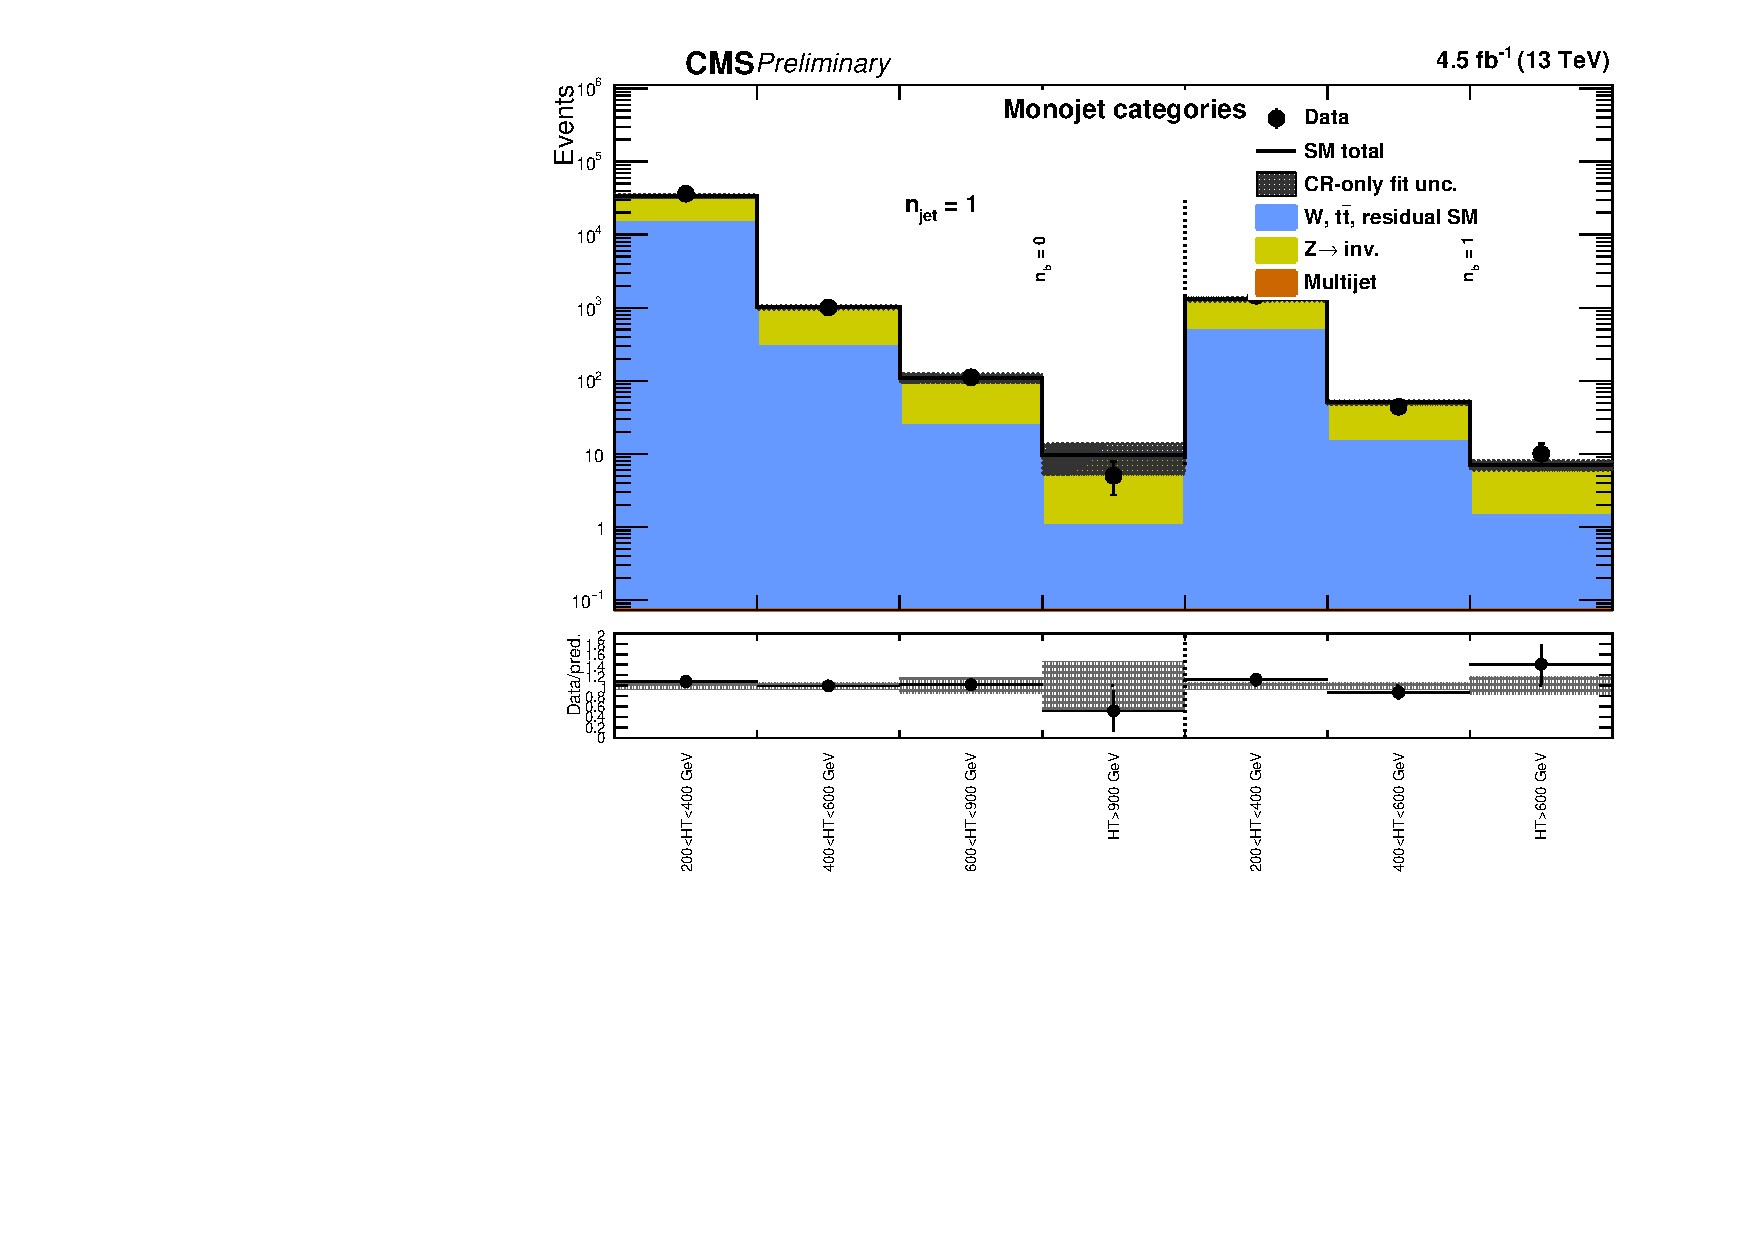
\includegraphics[width=1.\linewidth]{figures/results/mono/summaryPlot_Monojet_prefit}
\end{figure}

\clearpage
\begin{figure}[h!]
  \centering
  \caption{Upper panel. Event yields observed in data (solid circles)
    and SM expectations with their associated uncertainties (black
    histogram with shaded band) as a function of \nb and \scalht,
    integrated over \mht, and for the monojet category ($\njet = 1$)
    in the signal region. Lower panel. Data-to-background ratios. The
    background estimates and ratios are obtained with the full fit. }
  \label{fig:mr_mono_post}
  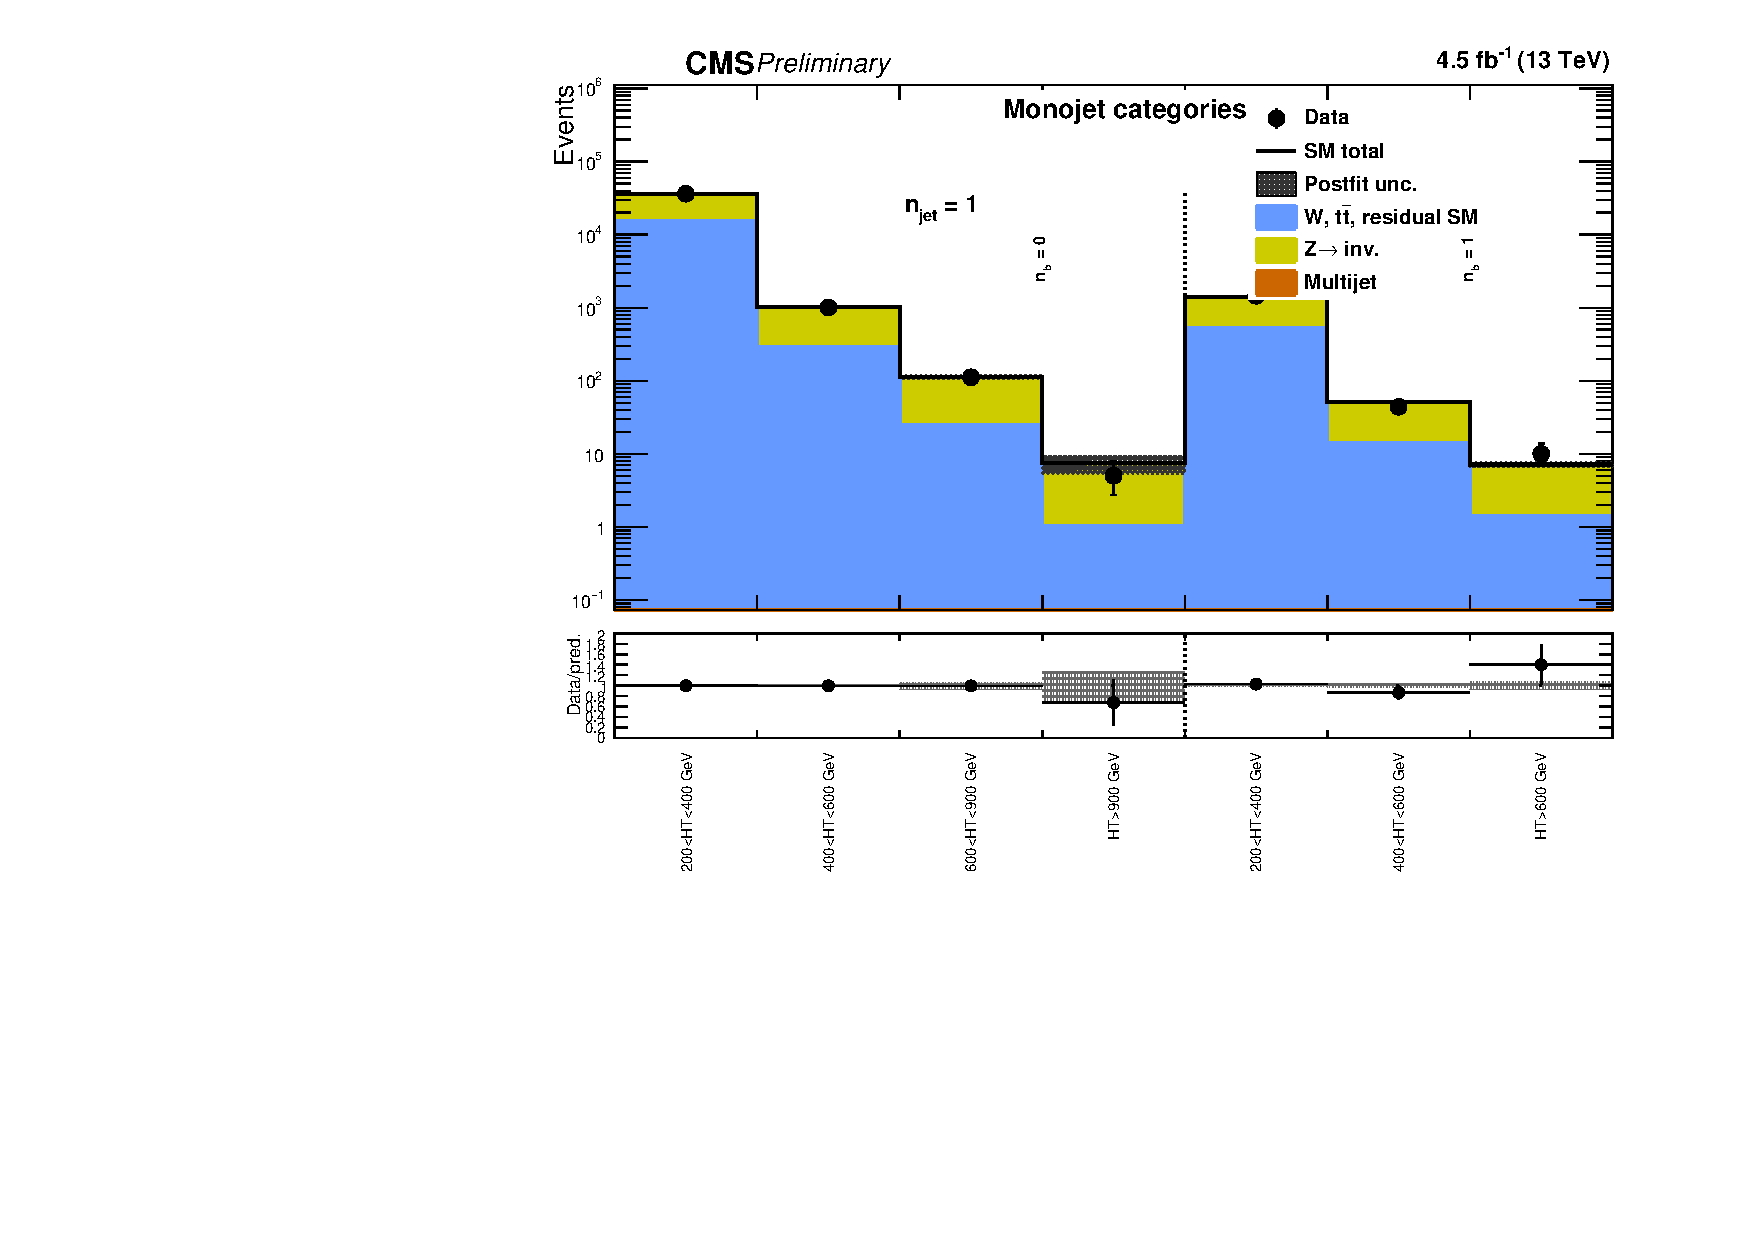
\includegraphics[width=1.\linewidth]{figures/results/mono/summaryPlot_Monojet_fit_b}
\end{figure}

\clearpage
\begin{figure}[h!]
  \centering
  \caption{Upper panel. Event yields observed in data (solid circles)
    and SM expectations with their associated uncertainties (black
    histogram with shaded band) as a function of \nb and \scalht,
    integrated over \mht, and for the monojet category ($\njet = 1$)
    in the signal region. Lower panel. The pulls, which are obtained
    from both the masked (red markers) and full (blue markers) fits. }
  \label{fig:mr_mono_pulls}
  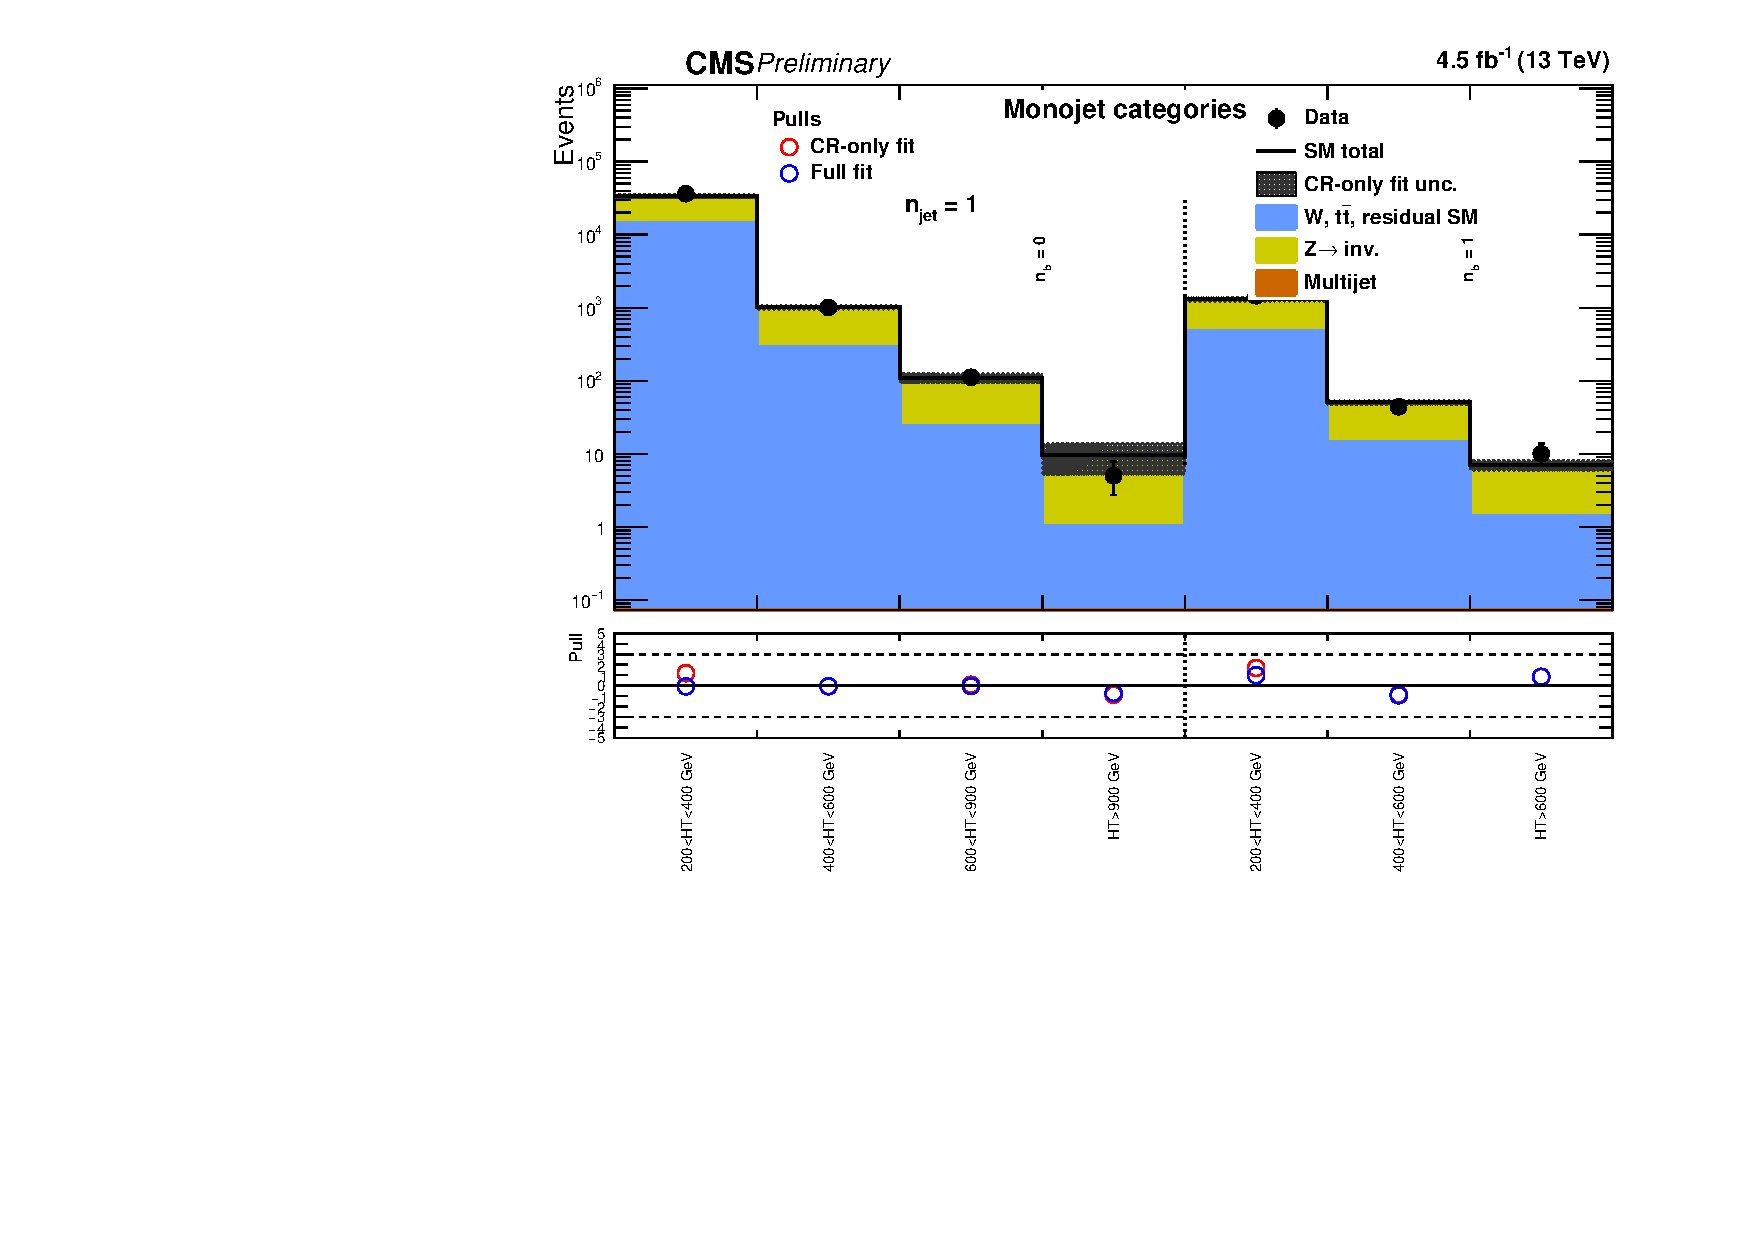
\includegraphics[width=1.\linewidth]{figures/results/mono/summaryPlot_Monojet_prefit_overlay_fit_b}
\end{figure}

% asym 

\clearpage
\begin{figure}[h!]
  \centering
  \caption{Upper panel. Event yields observed in data (solid circles)
    and SM expectations with their associated uncertainties (black
    histogram with shaded band) as a function of \nb and \scalht,
    integrated over \mht, and for the asymmetric \njet category
    in the signal region. Lower panel. Data-to-background ratios. The
    background estimates and ratios are from the masked fit. }
  \label{fig:mr_asym_pre}
  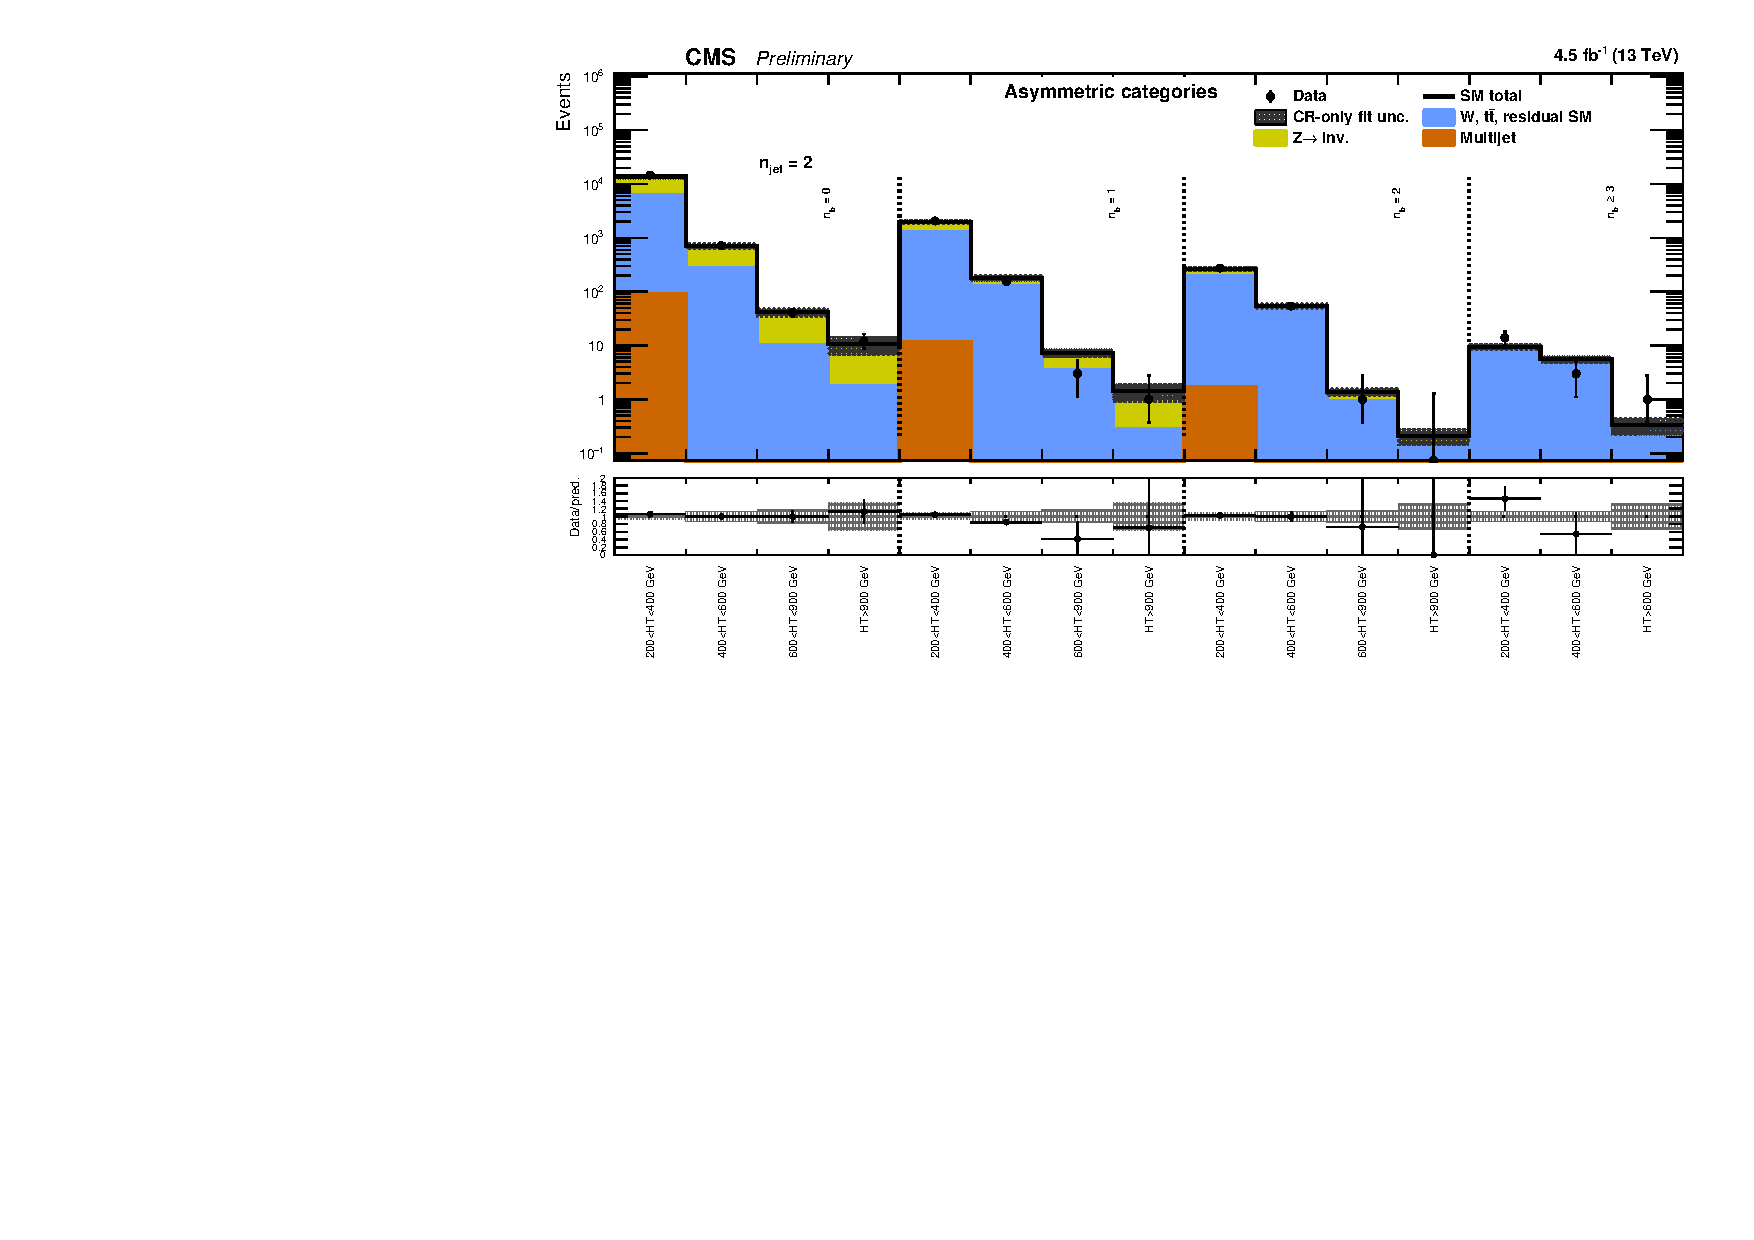
\includegraphics[width=1.\linewidth]{figures/results/asym/summaryPlot_Asymmetric_prefit}
\end{figure}

\clearpage
\begin{figure}[h!]
  \centering
  \caption{Upper panel. Event yields observed in data (solid circles)
    and SM expectations with their associated uncertainties (black
    histogram with shaded band) as a function of \nb and \scalht,
    integrated over \mht, and for the asymmetric \njet category
    in the signal region. Lower panel. Data-to-background ratios. The
    background estimates and ratios are obtained with the full fit. }
  \label{fig:mr_asym_post}
  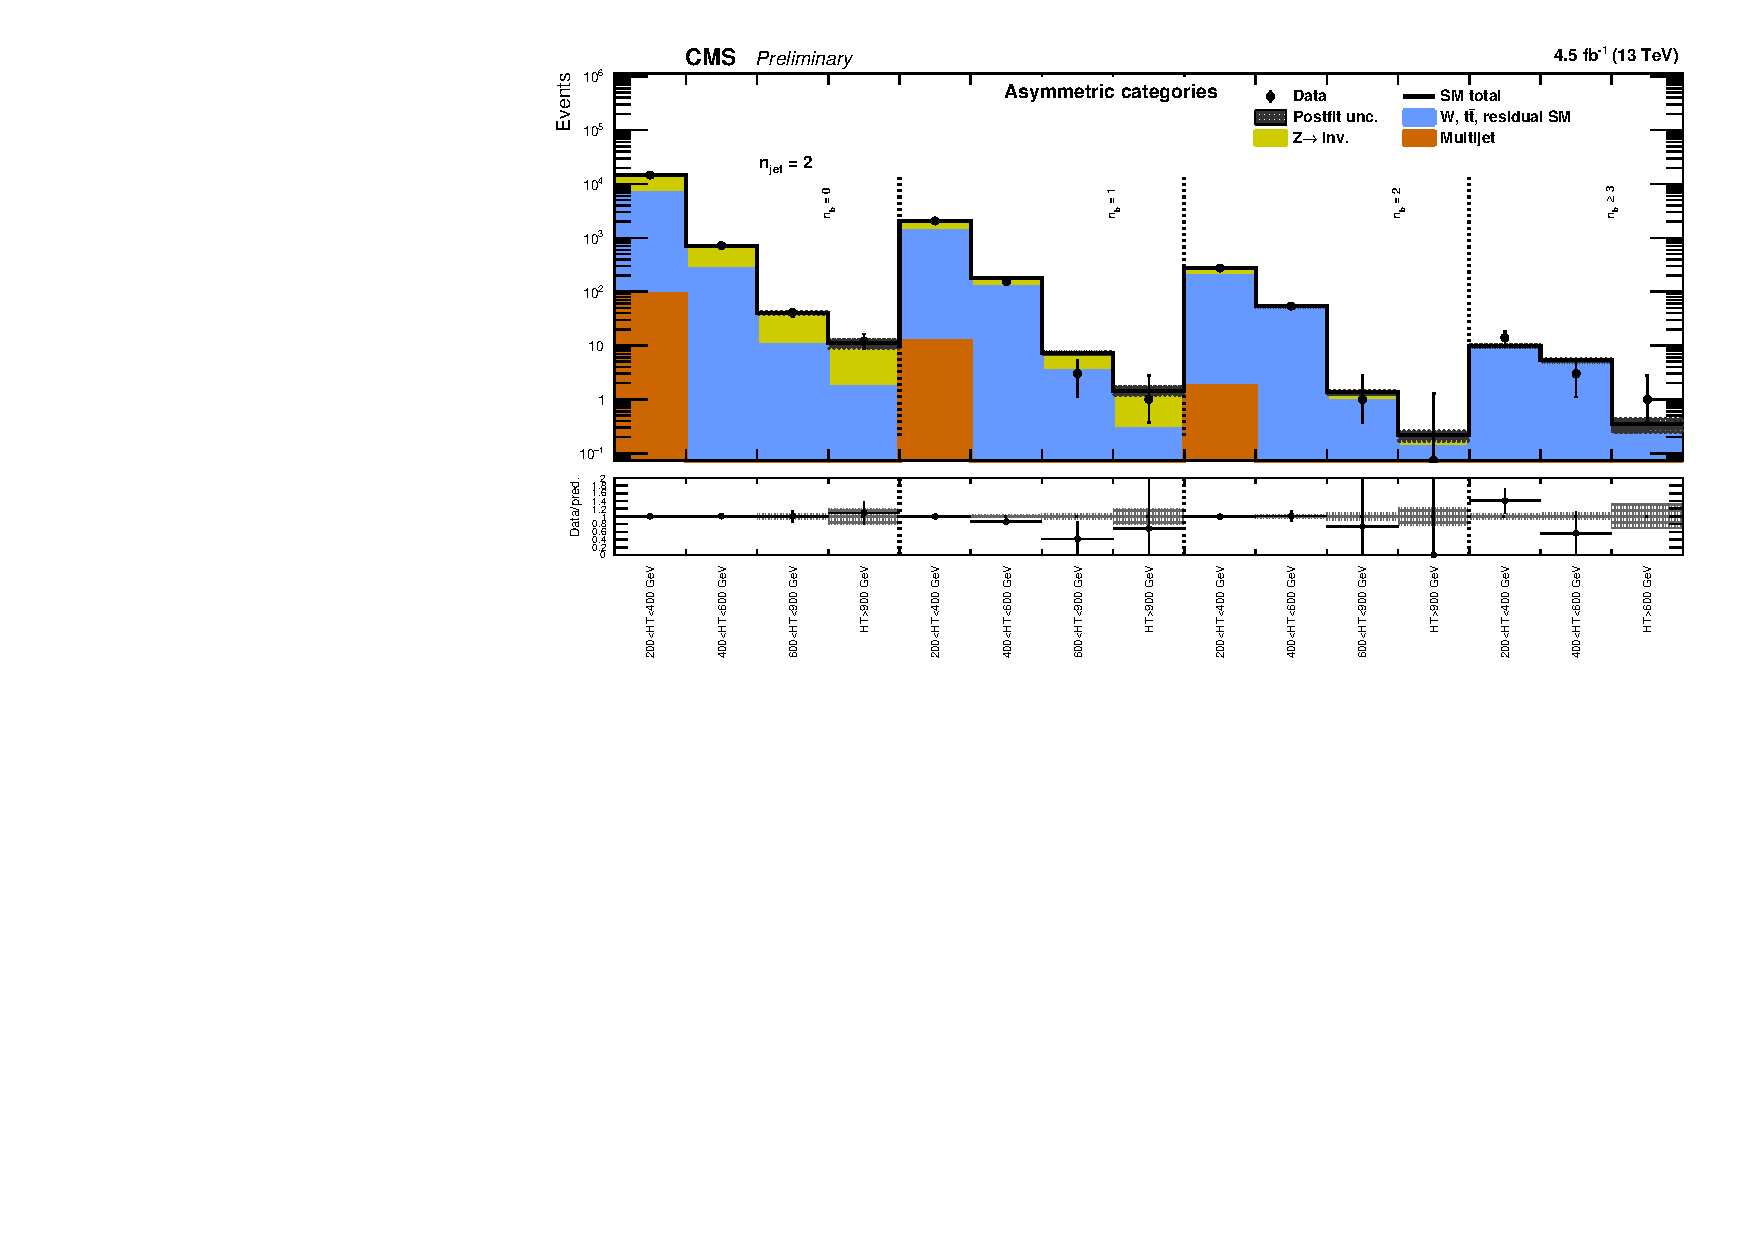
\includegraphics[width=1.\linewidth]{figures/results/asym/summaryPlot_Asymmetric_fit_b}
\end{figure}

\clearpage
\begin{figure}[h!]
  \centering
  \caption{Upper panel. Event yields observed in data (solid circles)
    and SM expectations with their associated uncertainties (black
    histogram with shaded band) as a function of \nb and \scalht,
    integrated over \mht, and for the asymmetric \njet category
    in the signal region. Lower panel. The pulls, which are obtained
    from both the masked (red markers) and full (blue markers) fits. }
  \label{fig:mr_asym_pulls}
  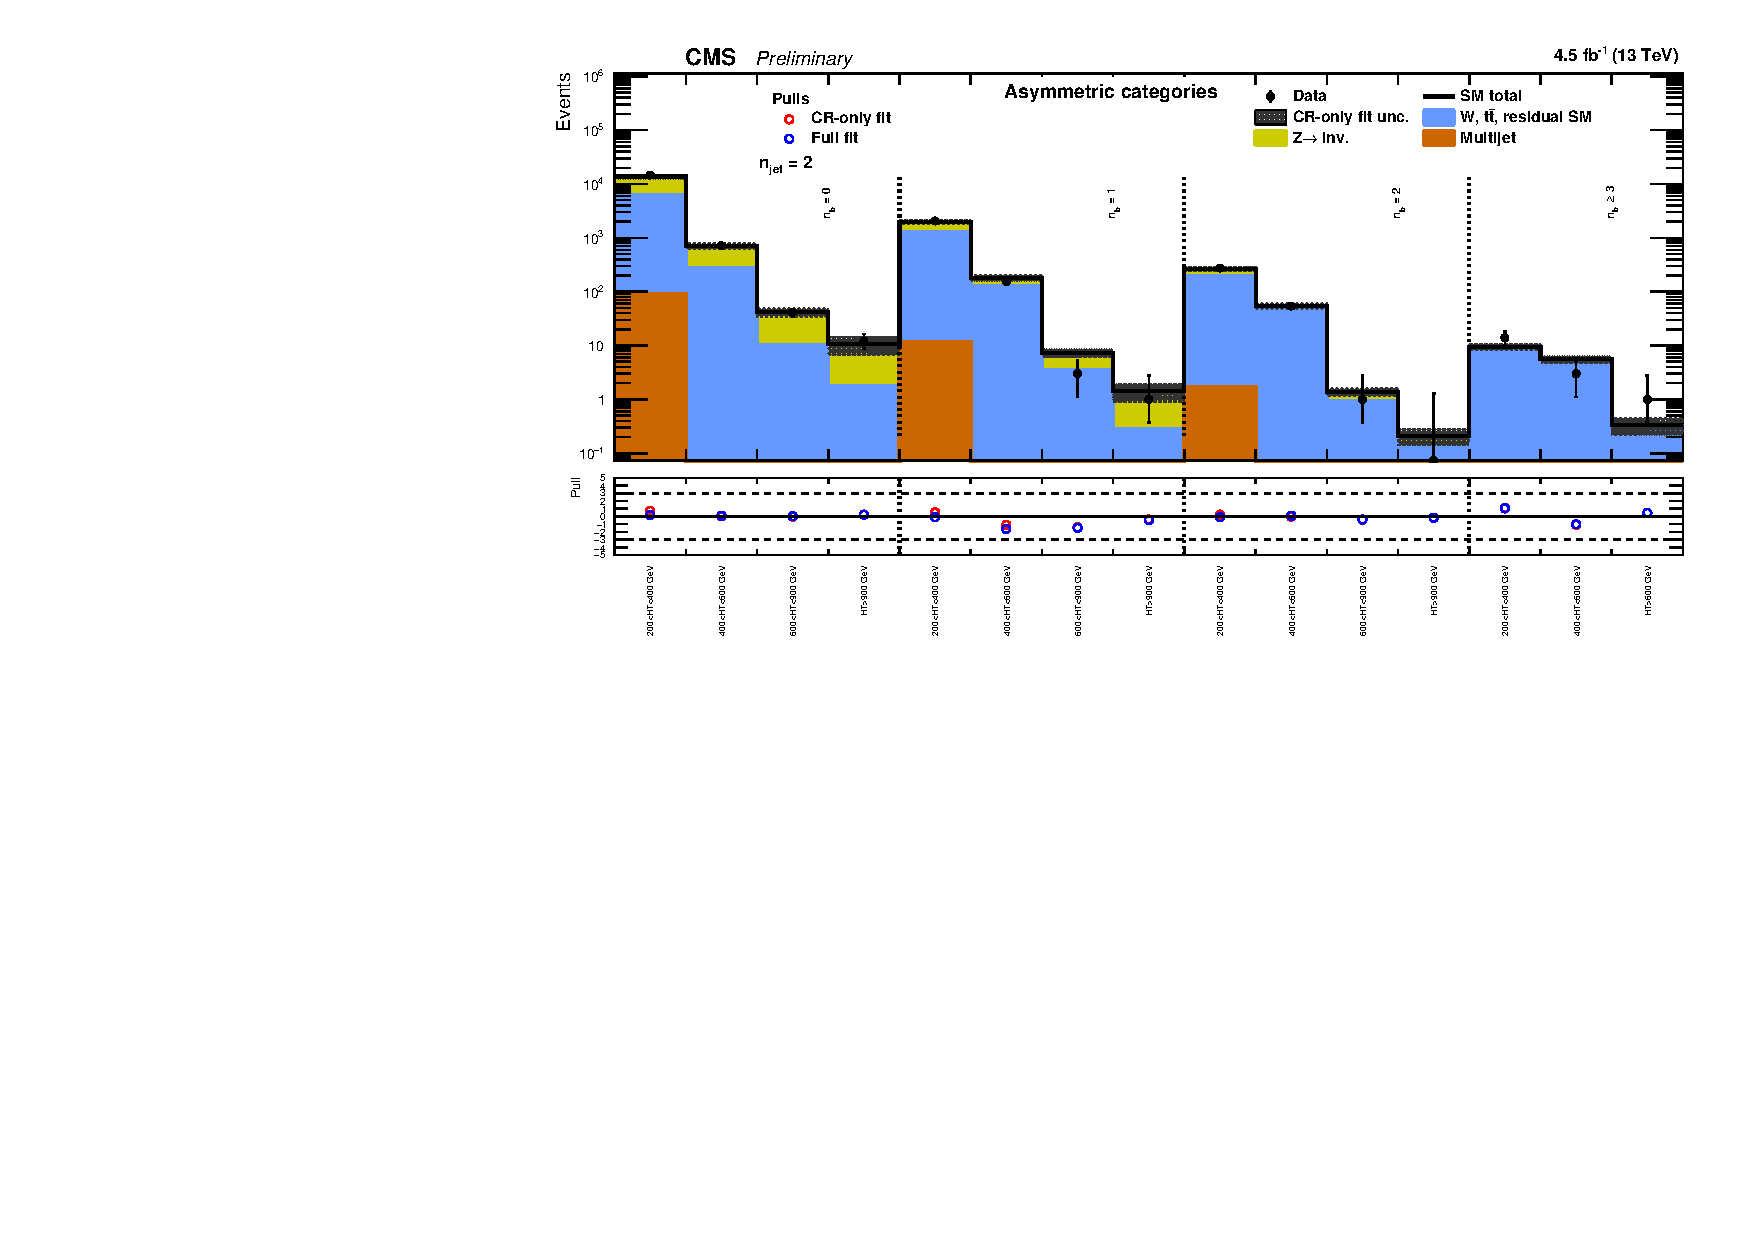
\includegraphics[width=1.\linewidth]{figures/results/asym/summaryPlot_Asymmetric_prefit_overlay_fit_b}
\end{figure}


% symm

\clearpage
\begin{figure}[h!]
  \centering
  \caption{Upper panel. Event yields observed in data (solid circles)
    and SM expectations with their associated uncertainties (black
    histogram with shaded band) as a function of \nb and \scalht,
    integrated over \mht, and for the symmmetric \njet category
    in the signal region. Lower panel. Data-to-background ratios. The
    background estimates and ratios are from the masked fit. }
  \label{fig:mr_symm_pre}
  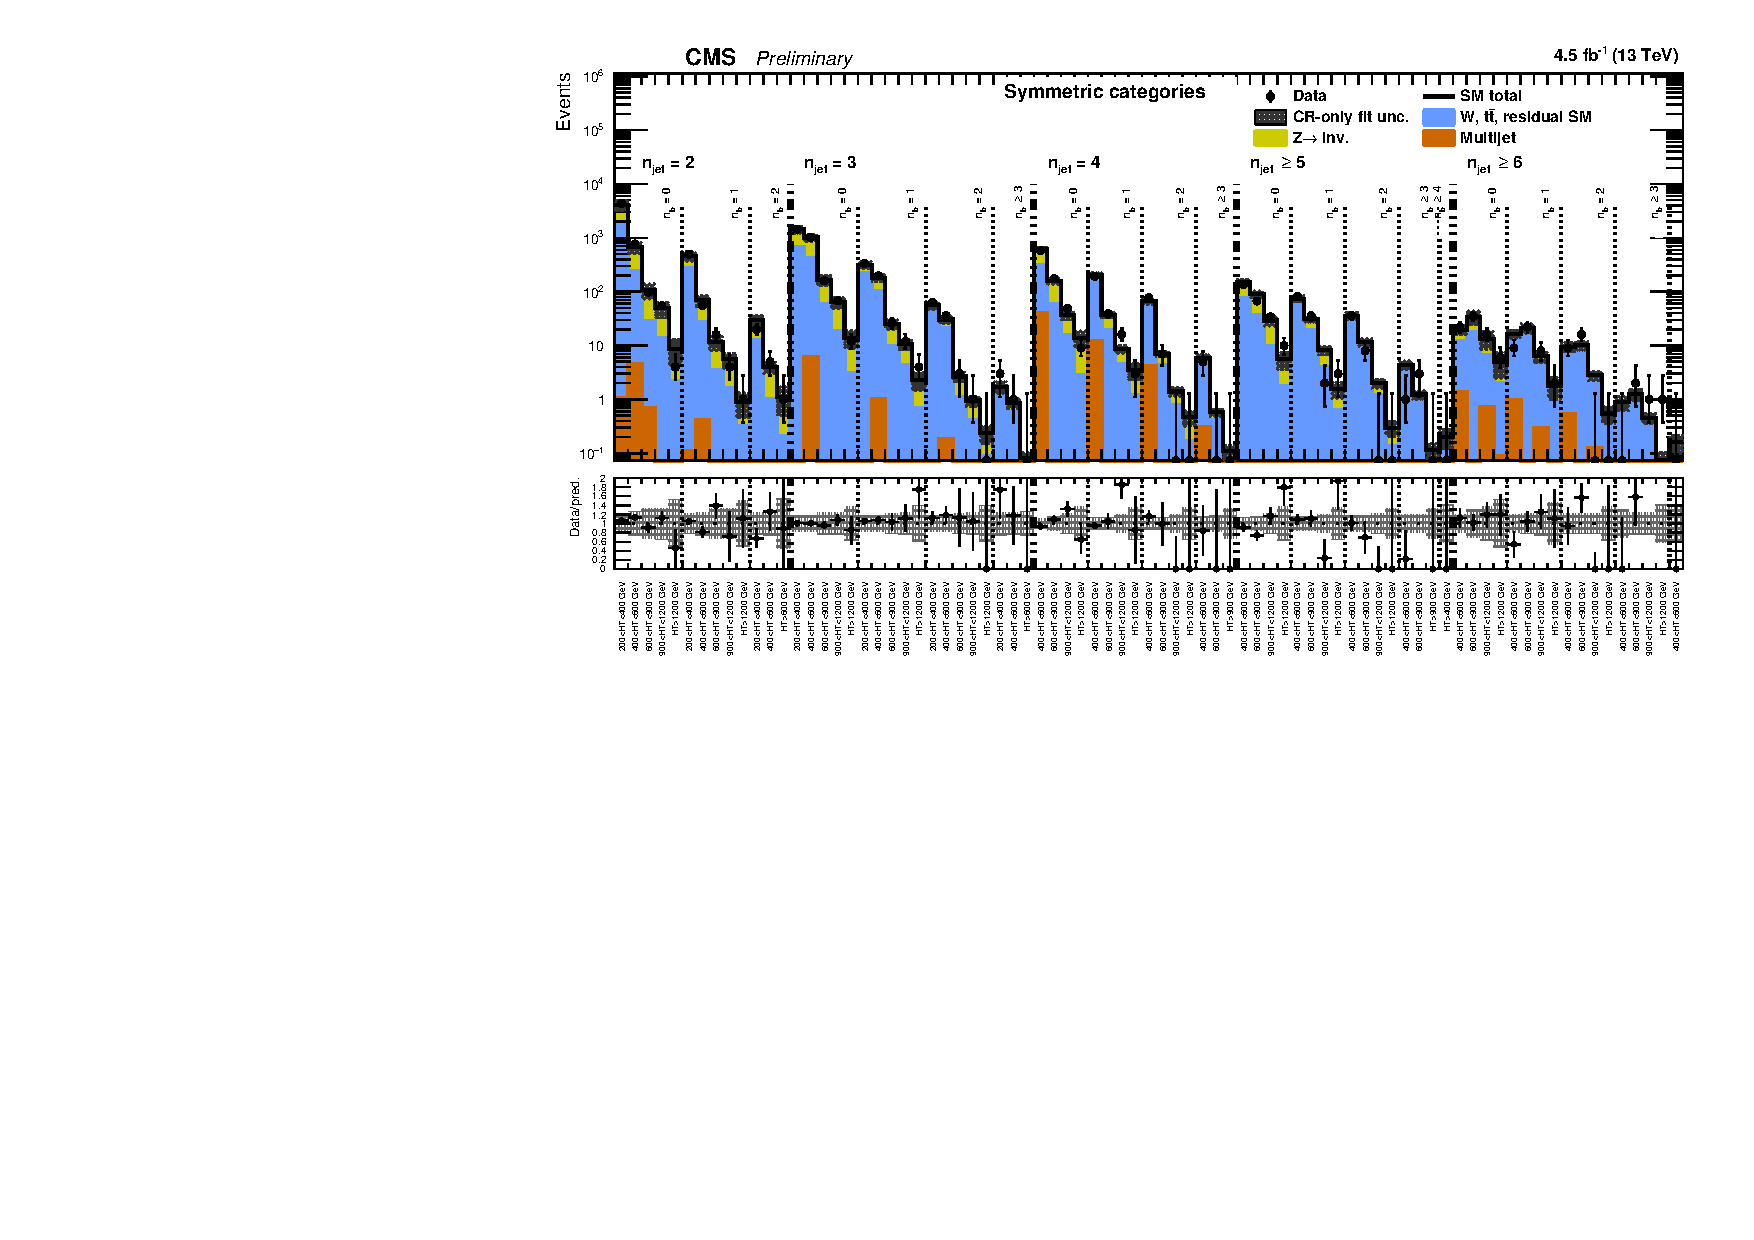
\includegraphics[width=1.\linewidth]{figures/results/symm/summaryPlot_Symmetric_prefit}
\end{figure}

\clearpage
\begin{figure}[h!]
  \centering
  \caption{Upper panel. Event yields observed in data (solid circles)
    and SM expectations with their associated uncertainties (black
    histogram with shaded band) as a function of \nb and \scalht,
    integrated over \mht, and for the symmmetric \njet category
    in the signal region. Lower panel. Data-to-background ratios. The
    background estimates and ratios are obtained with the full fit. }
  \label{fig:mr_symm_post}
  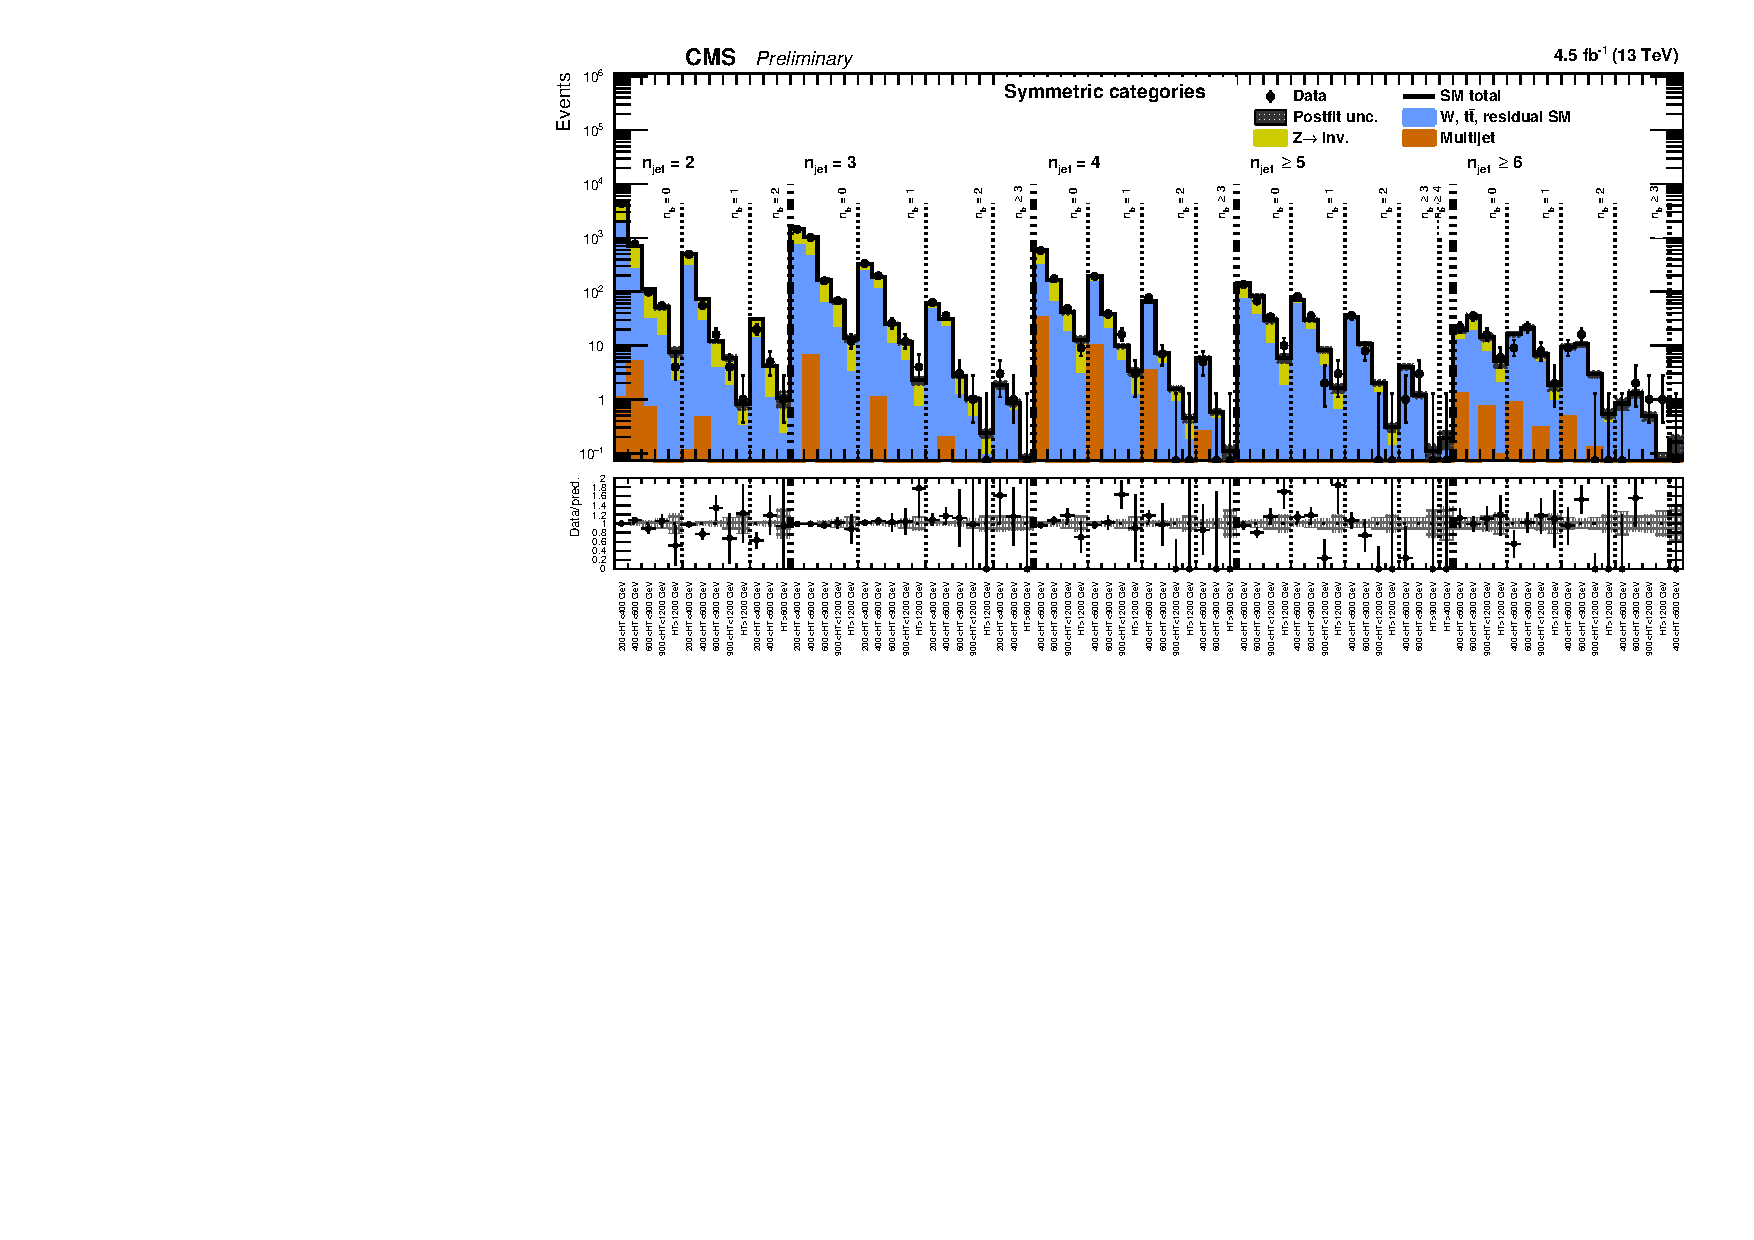
\includegraphics[width=1.\linewidth]{figures/results/symm/summaryPlot_Symmetric_fit_b}
\end{figure}

\clearpage
\begin{figure}[h!]
  \centering
  \caption{Upper panel. Event yields observed in data (solid circles)
    and SM expectations with their associated uncertainties (black
    histogram with shaded band) as a function of \nb and \scalht,
    integrated over \mht, and for the symmmetric \njet category
    in the signal region. Lower panel. The pulls, which are obtained
    from both the masked (red markers) and full (blue markers) fits. }
  \label{fig:mr_symm_pulls}
  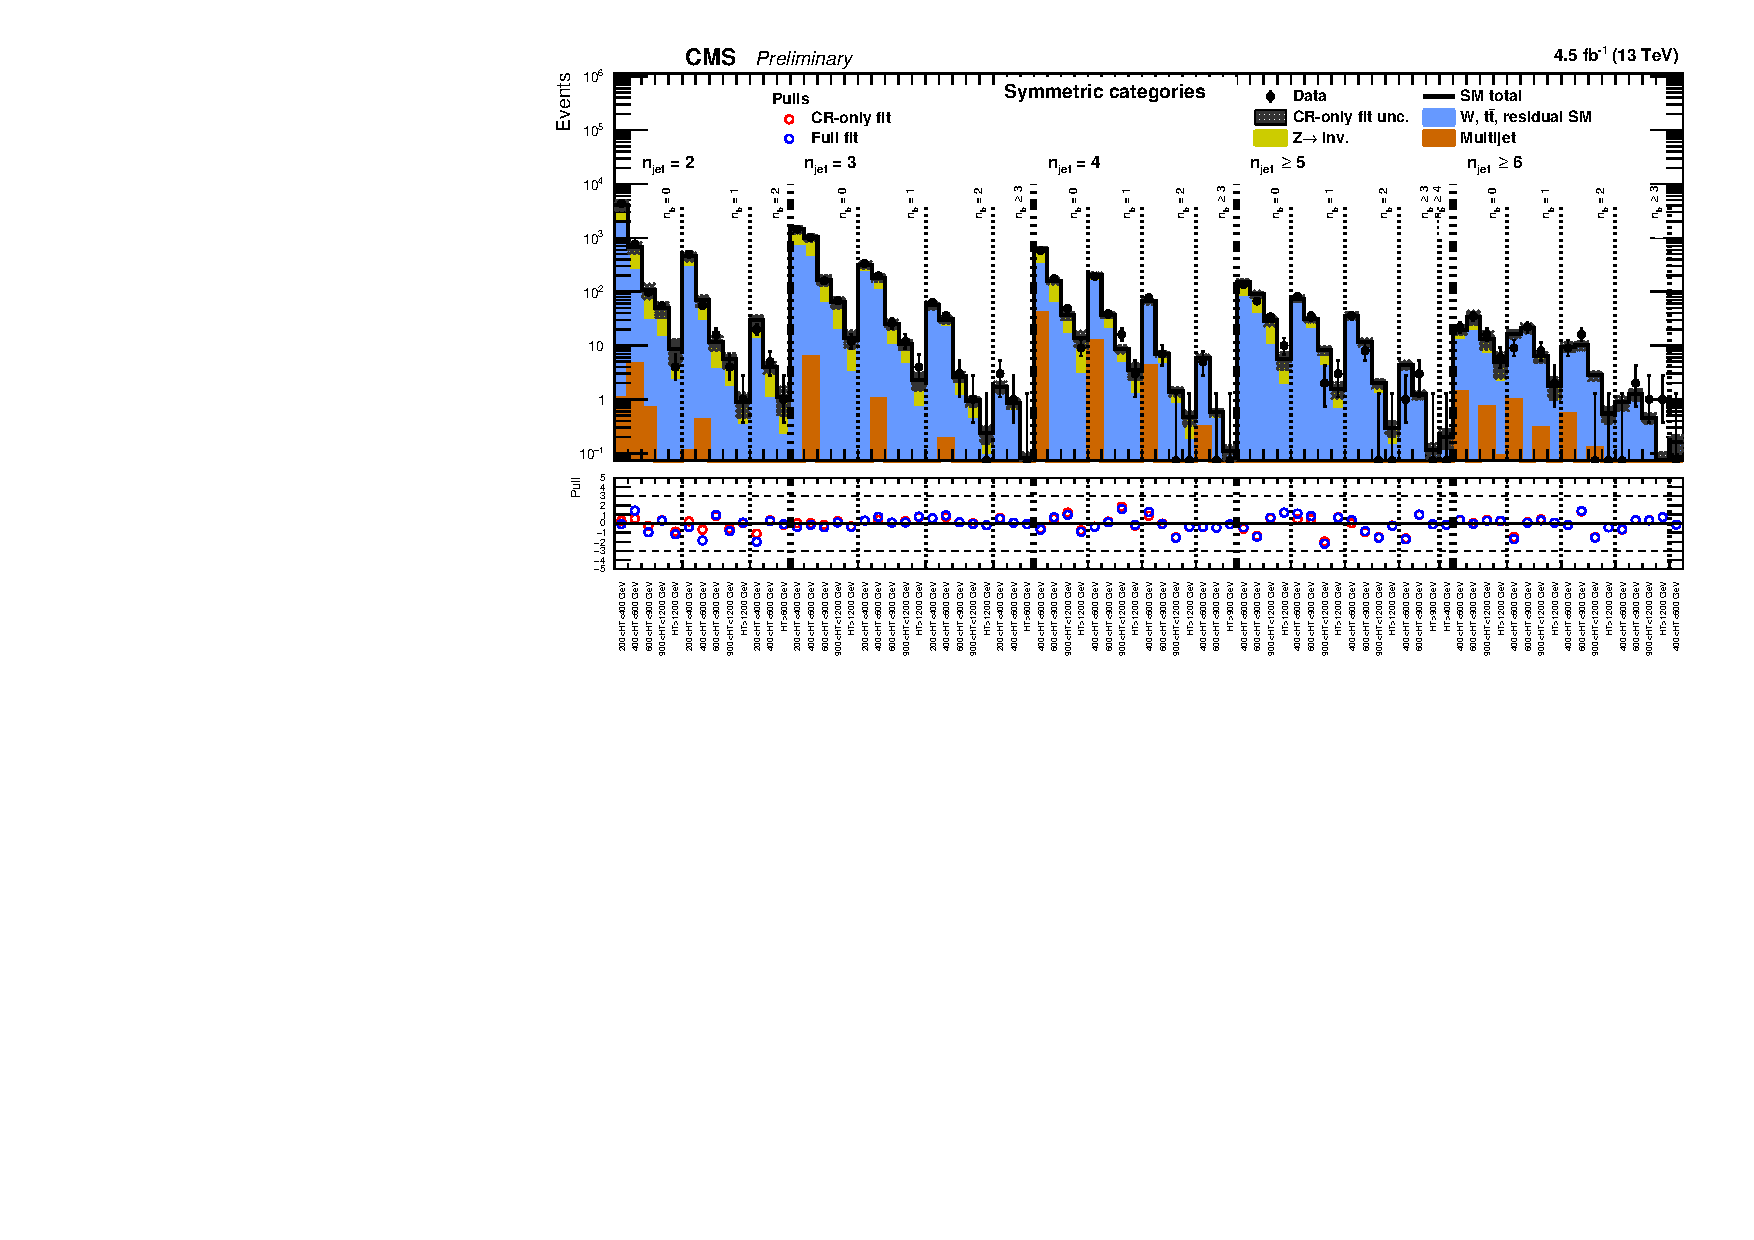
\includegraphics[width=1.\linewidth]{figures/results/symm/summaryPlot_Symmetric_prefit_overlay_fit_b}
\end{figure}

% 1d histograms 

\clearpage
\begin{figure}[h!]
  \centering
  \caption{(Left) Data-to-background ratios for the masked fit and all
    event categories. (Right) Pulls for the masked fit and all
    event categories.}
  \label{fig:ratios_and_pulls}
  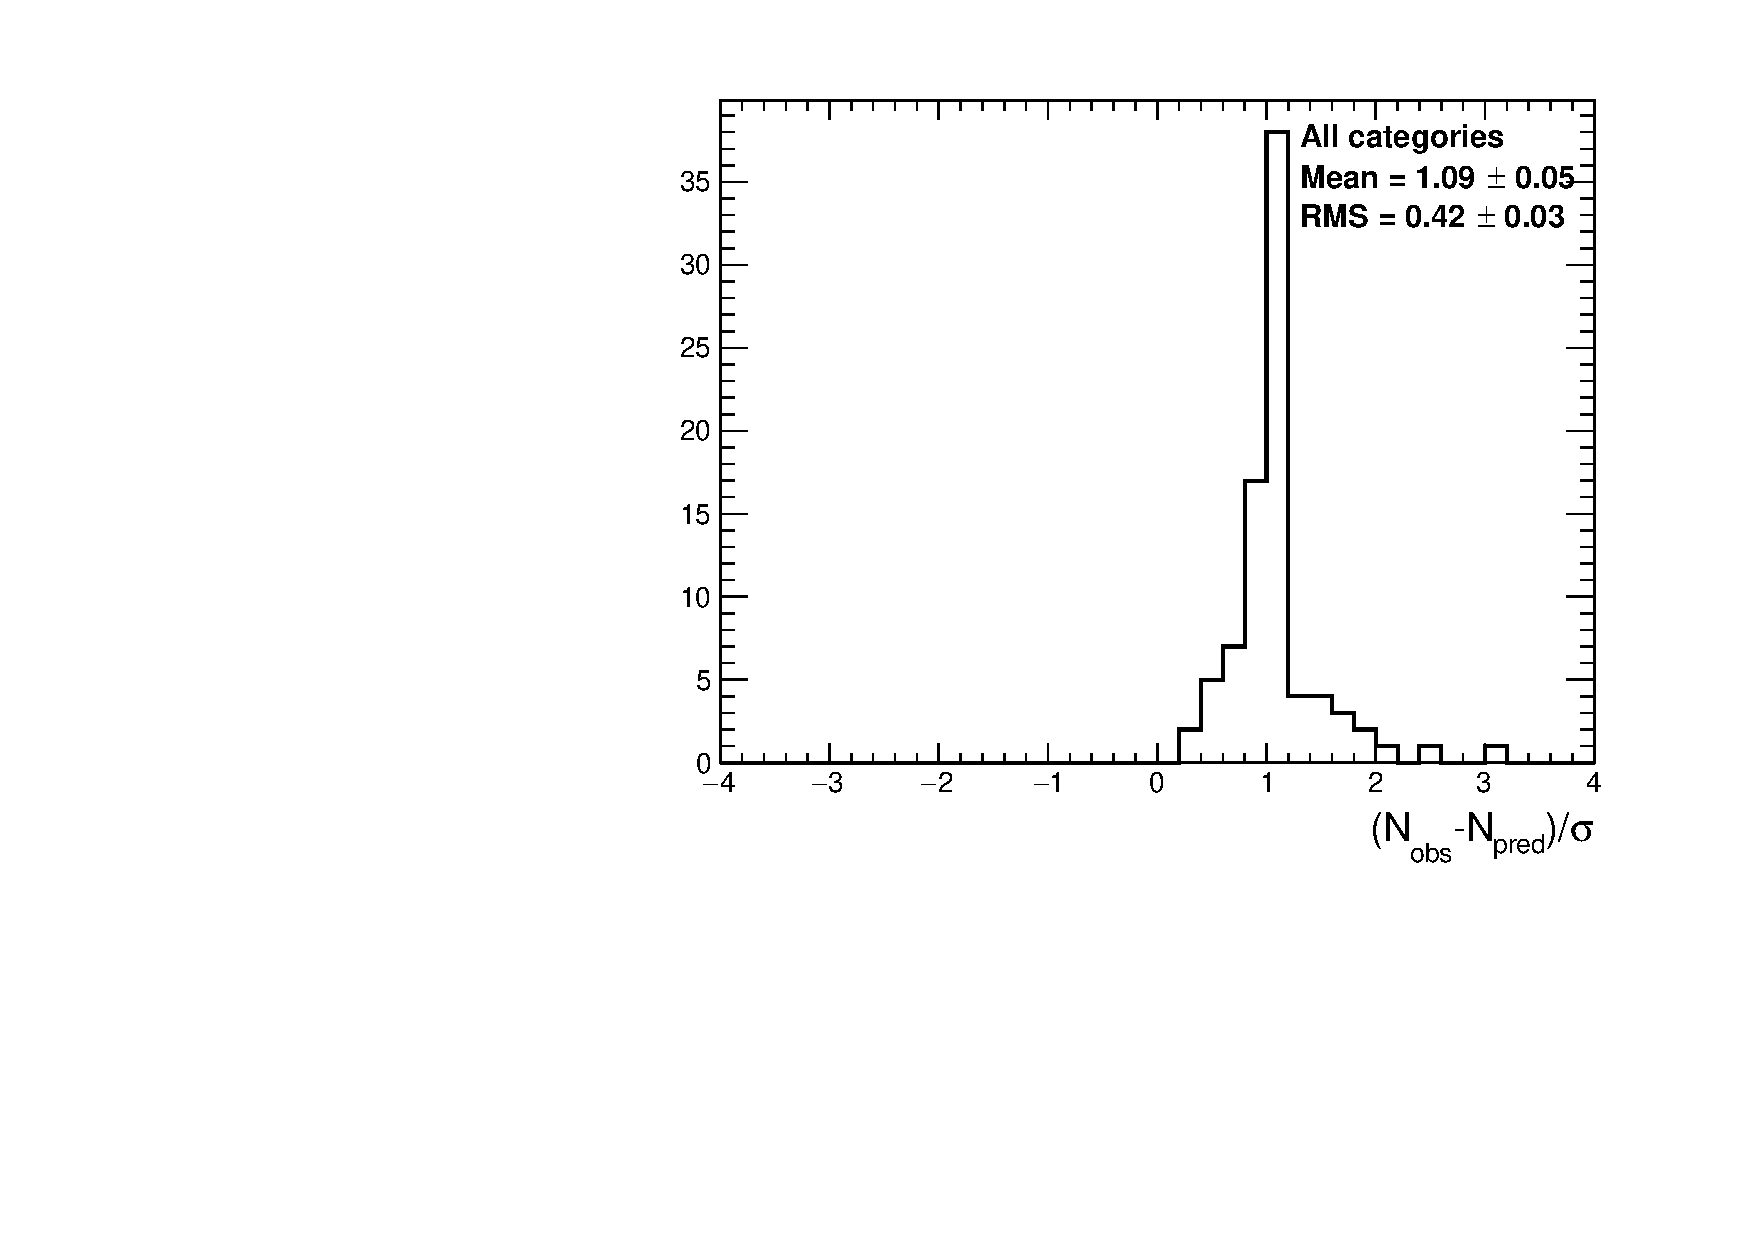
\includegraphics[width=0.49\linewidth]{figures/results/all/ratios_all_prefit.pdf}
  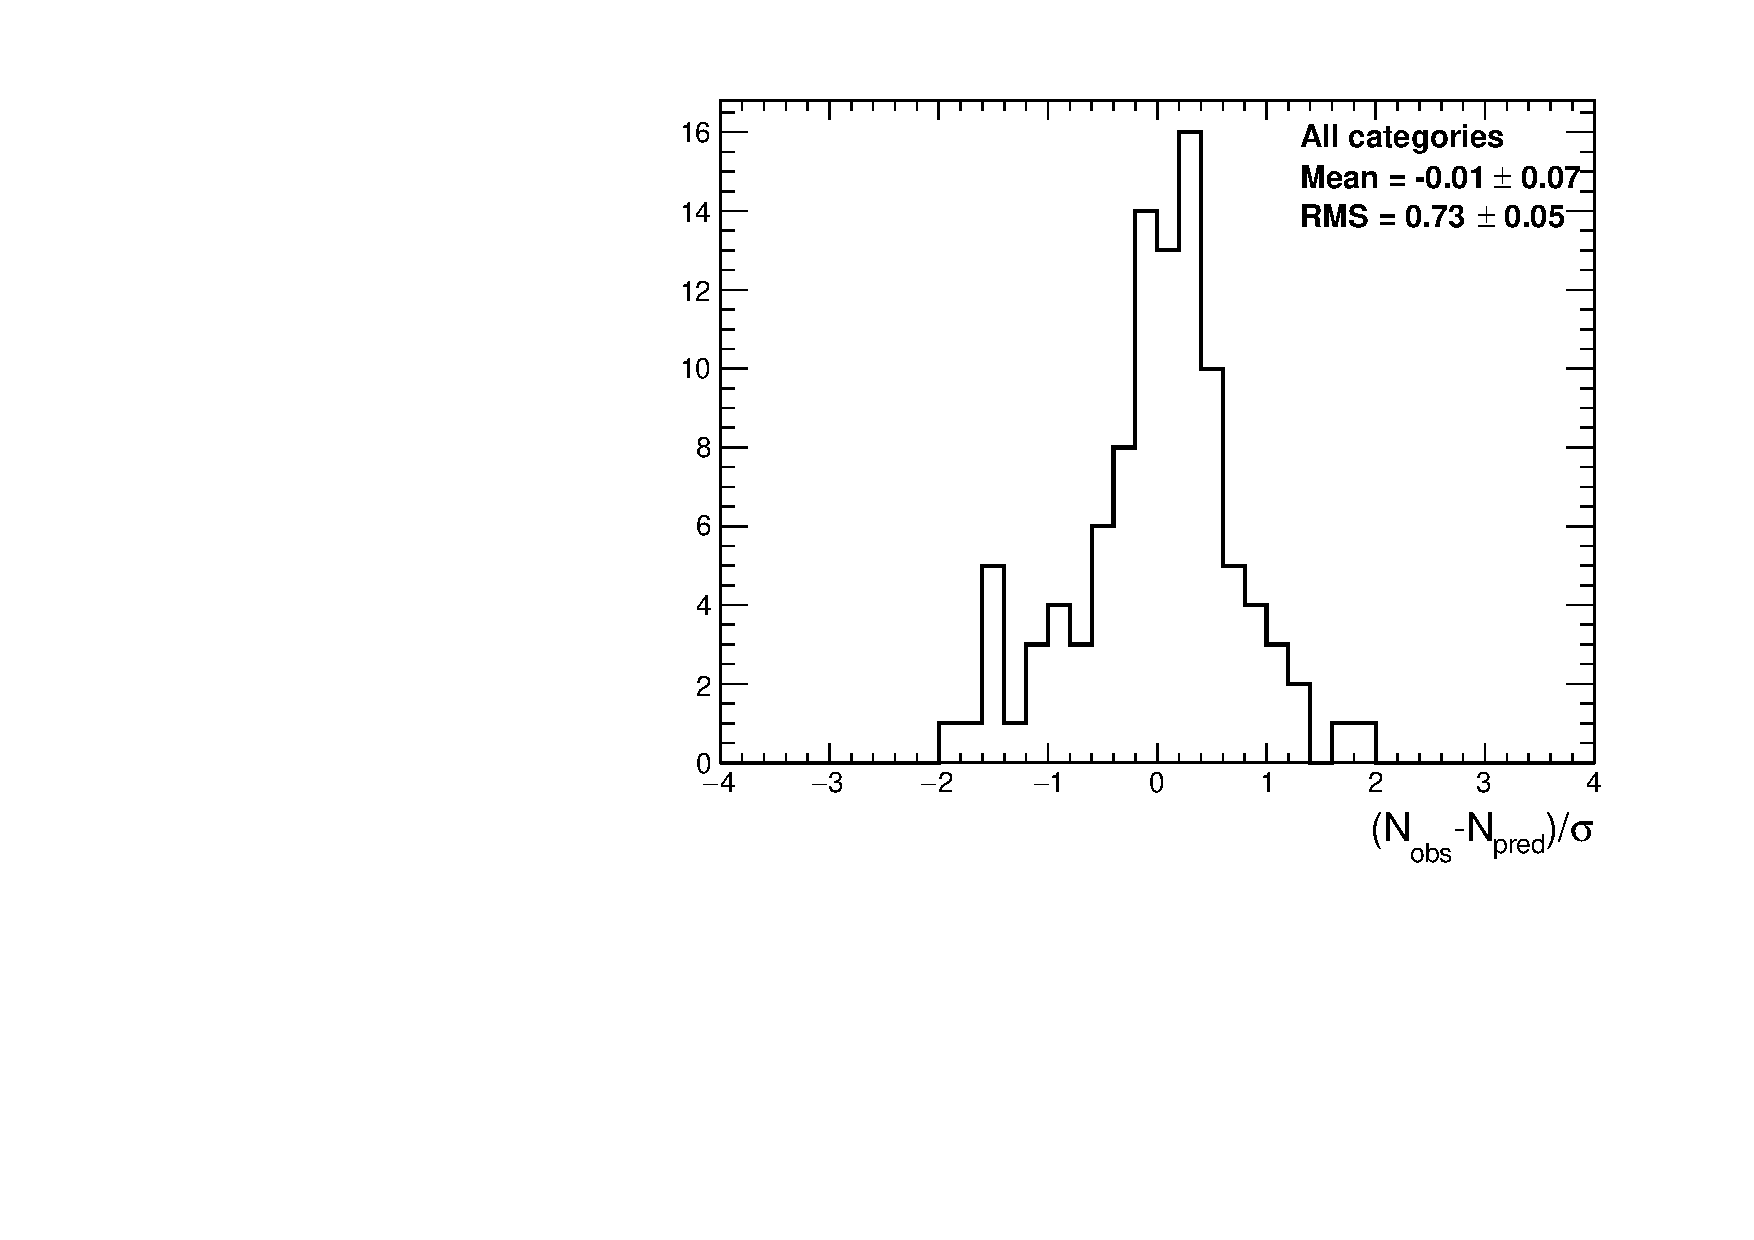
\includegraphics[width=0.49\linewidth]{figures/results/all/pulls_all_prefit.pdf}
\end{figure}

